\begin{frame}
	\frametitle{Interaktion Hydrosphäre, Kryosphäre und Atmosphäre}
	\begin{columns}
		\column{.6\linewidth}
		\begin{figure}
			\centering
			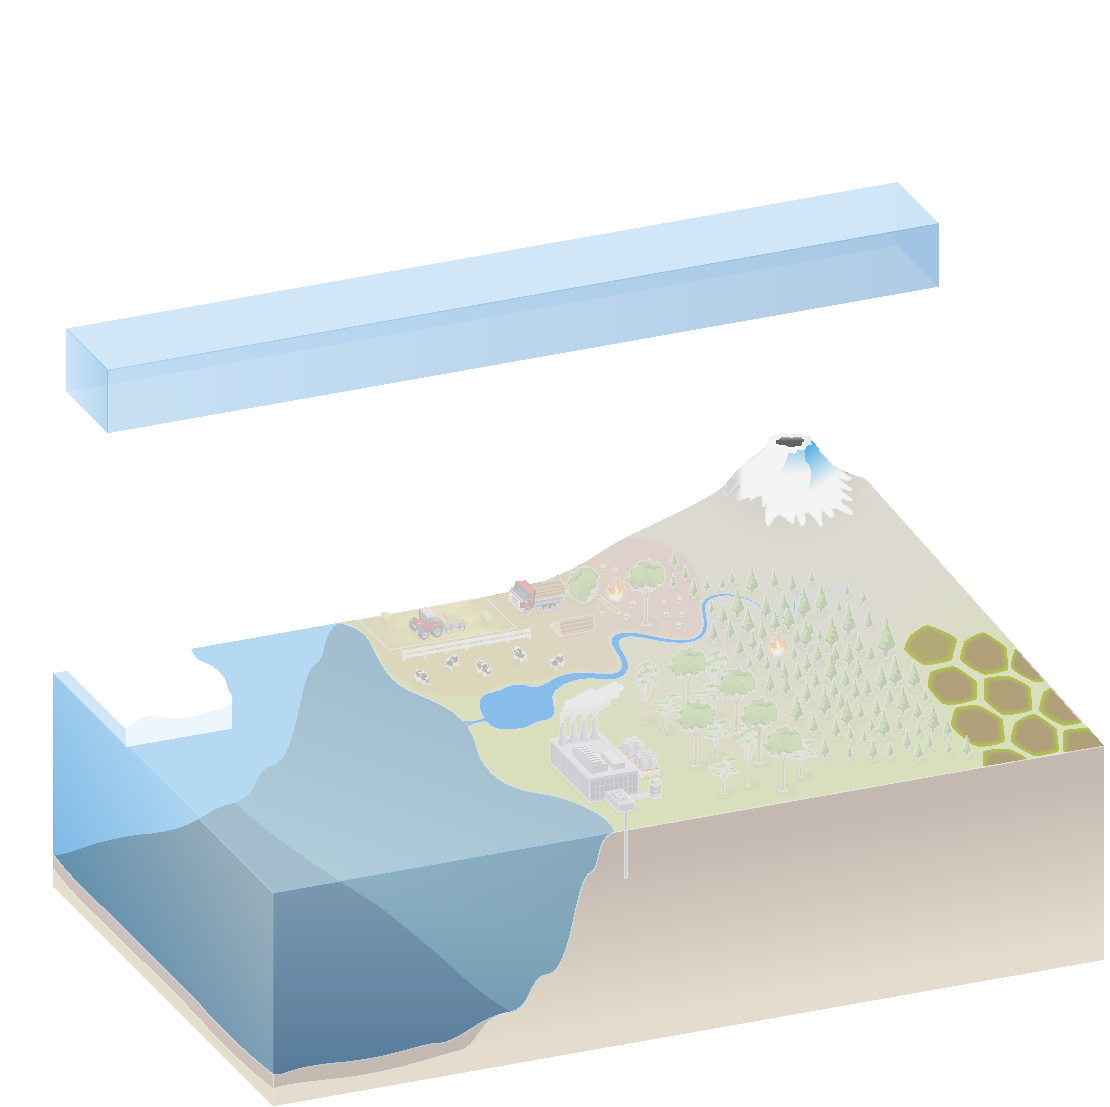
\includegraphics[trim={1cm 0cm 0cm 3cm}, clip, width=0.7\linewidth]{%
	        bilder/climate_components/global_climate_components_interaction_atmo_hydro_kryo.pdf}
			\caption{Interaktion Hydrosphäre, Kryosphäre und Atmosphäre}
		\end{figure}
		\column{.4\linewidth}
		\begin{itemize}
			\item Verringerter Albedo-Effekt
			\item Abgeschwächte Konvektion
			\item Abgeschwächte Ozeanströmung und Winde
			\item Anstieg des Meeresspiegels
			\item Massive Freisetzung von Treibhausgasen aus den Senken Ozean und Permafrost
			\item Trägheit führt zu verzögertem Eintreten der Änderungen
		\end{itemize}
	\end{columns}
	\begin{block}{}
			$\rightarrow$ Insgesamt: Eine Verstärkung des Treibhauseffekt mit weiteren noch unabsehbaren Folgen
	\end{block}

	\note{
		\begin{itemize}
			\item[] Verringerter Albedo-Effekt führt zu weniger Eis
			\item[] Wassermassen werden weniger stark abgekühlt, dadurch abgeschwächte Konvektion
			\item[] Ozeanströmungen und Winde werden ausgebremst
			\item[] Weniger Eis führt zu einem Anstieg des Meeresspiegels
			\item[] Massive Freisetzung von Treibhausgasen aus den Senken Ozean und Permafrost
			\item[] Trägheit führt zu verzögertem Eintreten der Änderungen
			\item[] Das Schmelzen der Polkappen und Auftauen des Permafrostes ist ein deutliches Signal
			\item[] Ein einmal in Gang gesetztes Abtauen kann schwer aufzuhalten sein
			\item[] Die Effekte können deutlich später auftreten (Trägheit der Klimakomponenten)
		\end{itemize}
	}
\end{frame}
